In this part of experiment, coil friction rig configuration is used and it will be used to calculate the coefficient of friction by varying the angle of lap. In addition to that, the slack tension is constant with 0.9 kg of mass and we keep increasing the load on the tight side until the coil belt starts to slip. The measurement experiment reading are shown on the table below:\\
\begin{table}[H]
\begin{center}
\begin{tabular}{|c|c|c|}
\hline
\begin{tabular}[c]{@{}c@{}}Angle \\ \\ (Radian)\end{tabular} & $M_2$ (kg) & $M_1$(kg)   \\ \hline
$\pi$/2                                                          & 0.9$\pm$0.1 & 1.27$\pm$0.1 \\ \hline
3$\pi$/2                                                         & 0.9$\pm$0.1 & 1.88$\pm$0.1 \\ \hline
4$\pi$/2                                                         & 0.9$\pm$0.1 & 2.8$\pm$0.1 \\ \hline
5$\pi$/2                                                         & 0.9$\pm$0.1 & 2.99$\pm$0.1 \\ \hline
6$\pi$/2                                                         & 0.9$\pm$0.1 & 3.44$\pm$0.1 \\ \hline
8$\pi$/2                                                         & 0.9$\pm$0.1 & 6.71$\pm$0.1 \\ \hline
\end{tabular}
\caption{Coil friction experiment results.}
\label{tab: 7}
\end{center}
\end{table}

According to the laboratory script, the ratio between natural logarithm of the tension side $\ln(T_1)$ and the natural logarithm of the slack side $\ln(T_2)$ is constant and it is equal to the product of the lap angle $\theta$ and the coefficient of friction $\mu$. Therefore, it is a linear relationship between tension side $\ln(T_1)$ and  slack side $\ln(T_2)$ and the linear equation is:
\begin{equation}
\ln(T_1) = \mu\theta + \ln(T_2)
\end{equation}
The tension force on each side is equal to the weight force $F_g$ and it is given by $m*g$ where $m$ is the mass of the object and $g$ is the acceleration due to gravity. Since we conduct this experiment on the same location as the moment of inertia experiment, then we can use the same value for the acceleration due to gravity. In addition to that, the uncertainty to tension force of is given by:
\begin{align}
\delta T&=\pm \abs{\left(g\right)(\delta m)} + \abs{\left(m\right)(\delta g)} \notag
\end{align}
The tension for both the slack side and the tight side are given on the table below:
\begin{table}[H]
\begin{center}
\begin{tabular}{|c|c|c|}
\hline
\begin{tabular}[c]{@{}c@{}}Angle \\ (Radian)\end{tabular} & $T_2$ (N)   & $T_1$(N)      \\ \hline
$\pi$/2                                                          & 8.81$\pm$0.98 & 12.44$\pm$0.98  \\ \hline
3$\pi$/2                                                         & 8.81$\pm$0.98 & 18.41$\pm$0.981 \\ \hline
4$\pi$/2                                                         & 8.81$\pm$0.98 & 27.4$\pm$0.982  \\ \hline
5$\pi$/2                                                         & 8.81$\pm$0.98 & 29.28$\pm$0.982 \\ \hline
6$\pi$/2                                                         & 8.81$\pm$0.98 & 33.69$\pm$0.983 \\ \hline
8$\pi$/2                                                         & 8.81$\pm$0.98 & 65.72$\pm$0.986 \\ \hline
\end{tabular}
\caption{Coil tension.}
\label{tab: 8}
\end{center}
\end{table}

Taking the natural logarithm for both $T_2$ and $T_1$, then:
\begin{table}[H]
\begin{center}
\begin{tabular}{|c|c|c|}
\hline
\begin{tabular}[c]{@{}c@{}}Angle \\ (Radian)\end{tabular} & $\ln(T_2)$   & $\ln(T_1)$      \\ \hline
$\pi$/2                                                          & 2.78$\pm$-0.02 & 2.52$\pm$-0.02  \\ \hline
3$\pi$/2                                                         & 2.78$\pm$-0.02 & 2.91$\pm$-0.019 \\ \hline
4$\pi$/2                                                         & 2.78$\pm$-0.02 & 3.31$\pm$-0.018  \\ \hline
5$\pi$/2                                                         & 2.78$\pm$-0.02 & 3.38$\pm$-0.0182 \\ \hline
6$\pi$/2                                                         & 2.78$\pm$-0.02 & 3.52$\pm$-0.0171 \\ \hline
8$\pi$/2                                                         & 2.78$\pm$-0.02 & 4.19$\pm$-0.0141\\ \hline
\end{tabular}
\caption{Natural logarithmic of the coil tension.}
\label{tab: 9}
\end{center}
\end{table}

Plotting the equilibrium values of $\ln(T_1)$ versus $\theta$ and setting the intercept to 2.78, the outputted graph is shown below:
 \begin{figure}[H]
\centering
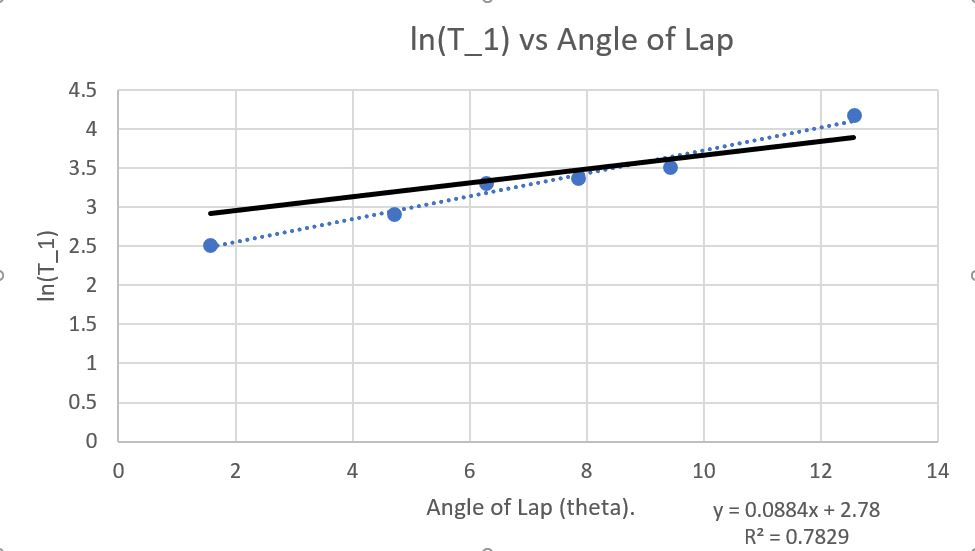
\includegraphics[width=1\textwidth]{chapters/lab2/graph1}
\caption{Equilibrium values of $\ln(T_1)$ vs $\theta$.}
\label{fig:mesh2}
\end{figure}
Drawing the line of best fit from the y-intercept then the equation of the line in terms of $\theta$ and $\ln(T_1)$ is given by:
\begin{equation}
\ln(T_1) = 0.0884\theta + 2.78 
\end{equation}

Therefore, the coefficient of friction $\mu$ is approximately 0.0884.

